\subsection{Information for judges}

\center{\large{\textbf{Team PML30-Y (FTC-15)}}} \newline

The basic principle we followed in engineering is modular. Our robot was divided into several modules and for every module there was appointed a responsible person from the team members. There are 4 main modules in our robot. They are:

\begin{enumerate*}
	
	\item Wheel base - a system that provides movement of the robot. Responsible - Gordei Kravtsov.
	
	\item Gripper - a system for collecting debris. Responsible - Andrew Nemov.
	
	\item Bucket - a system for keeping debris until it will be put into a goal. Responsible - Aleksandr Iliasov.
	
	\item Elevator - a system for delivering the bucket to middle and top goals of the mountains. Responsible - Nikita Safronov.
	
\end{enumerate*}

In our technical documentation there is a special section named "Specifications for modules" which is dedicated to the development process of modules in particular. In this section you can find more information about modules mentioned above.

Software specifications are available in section named "Specifications for programs".

General development of the robot in progress is represented in chronological section. This section contains information about all the team meetings including discussions and days of competitions (it mentioned in the title of meeting).

Our abilities and our strategy in the game are provided in section "Key summary".

In the section "Appendix" you can find":
\begin{enumerate*}
	\item The list of raw materials used in robot.
	
	\item The example of leaflet with our robot's characteristics that we intend to distribute among other teams to make them know about our abilities.
	
	\item The information list for judges (which you are reading right now).
	
\end{enumerate*}

You can learn more about the structure of our technical book in the section "How to read this book".

\begin{figure}[H]
	\begin{minipage}[h]{0.35\linewidth}
		\center{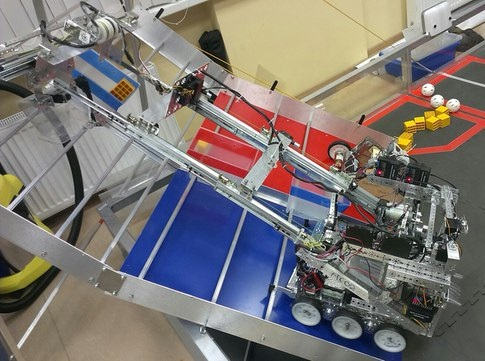
\includegraphics[scale = 0.35]{4Appendix/7Leaflet_for_judges/images/01}}
	\end{minipage}
	\hfill
	\begin{minipage}[h]{0.35\linewidth}
		\center{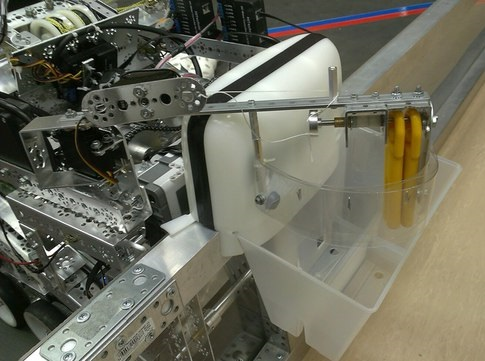
\includegraphics[scale = 0.35]{4Appendix/7Leaflet_for_judges/images/02}}
	\end{minipage}
	\hfill
	\begin{minipage}[h]{0.25\linewidth}
		\center{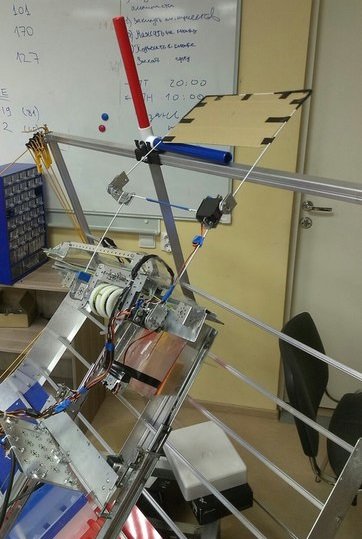
\includegraphics[scale = 0.3]{4Appendix/7Leaflet_for_judges/images/03}}
	\end{minipage}
\end{figure} 